\section{3D Video Chat}\label{sec:3d-video-chat}

Google's Project Starline~\cite{lawrence_project_2021} (Figure~\ref{fig:google-starline}) is state-of-the-art in 3D video chatting. It is a real-time bidirectional communication system that lets two distant users experience a conversation as if they were copresent. Despite being state-of-the-art, Project Starline is as yet unable to allow for more than a single participant to be present at either end of the line. While there may still be a ways to go before such a high-fidelity telepresence system can cater to more than two participants at a time, there are numerous breakthroughs that Project Starline has achieved so far and will continue to achieve with further prototype refinements/overhauls.

There has been a considerable amount of work~\cite{google_ar__vr_project_2021} in the area of 3D video chatting over the past 30 years, and prior research systems have been described that also use freestanding displays and depth sensors. Some of these include 2011's Maimone and Fuchs~\cite{maimone_encumbrance-free_2011}, 2013's Zhang et al.~\cite{zhang_viewport_2013}, and 2009's Jones et al.~\cite{jones_achieving_2009}. More recent work has investigated head-mounted displays for telepresence applications, including the Holoportation project~\cite{orts-escolano_holoportation_2016} from Microsoft Research in 2016. And more recently, the line of research on codec avatars~\cite{chu_expressive_2020} is being pursued at Facebook Reality Labs.

The Project Starline system~\cite{google_ar__vr_project_2021} (Figure~\ref{fig:starline-data-flow}) combines an autostereoscopic display with a real-time 3D capture and real-time 3D audio pipeline to present the remote person as they truly are, including faithfully reproducing important nonverbal cues like eye contact. Their display and setup achieve a retina resolution of 45 pixels per degree across the target field of view, showing the other person in greater detail than is currently possible with today's state-of-the-art VR headsets and AR glasses. Either participant sits on a bench that is connected to a large infrared backlight located directly behind them. And they see their conversation partner through a 60-hertz 65-inch 8K autostereoscopic display located roughly 1.2 meters in front of them. This display conveys both stereo and parallax cues to the seated participant and shows the remote person at their true physical size. They use four face-tracking cameras running at 120 frames per second to steer this display to the viewer's eyes. These estimate the 3D location of the eyes, ear, and mouth within about 5 millimeters of precision. They use a fast face tracker to find 2D spatial features and triangulate to find the 3D locations. These are used to render the appropriate viewpoints to steer the 3D display and to drive free-space spatialized 3D audio. The spatialized audio system uses two speakers and an array of four microphones. On the input side, face tracking data enables dynamic beamforming, sharpening the microphones' directionality to combat noise and reverberation. On the output side, tracking enables the system to spatialize playback at the location of the speaker's mouth. Tracking also enables binaural crosstalk cancellation to target the correct waveforms at the listener's ears. Thus, even though the speakers are spaced far apart, the sound appears to emanate from the remote user's mouth.

\begin{figure}[!h]
    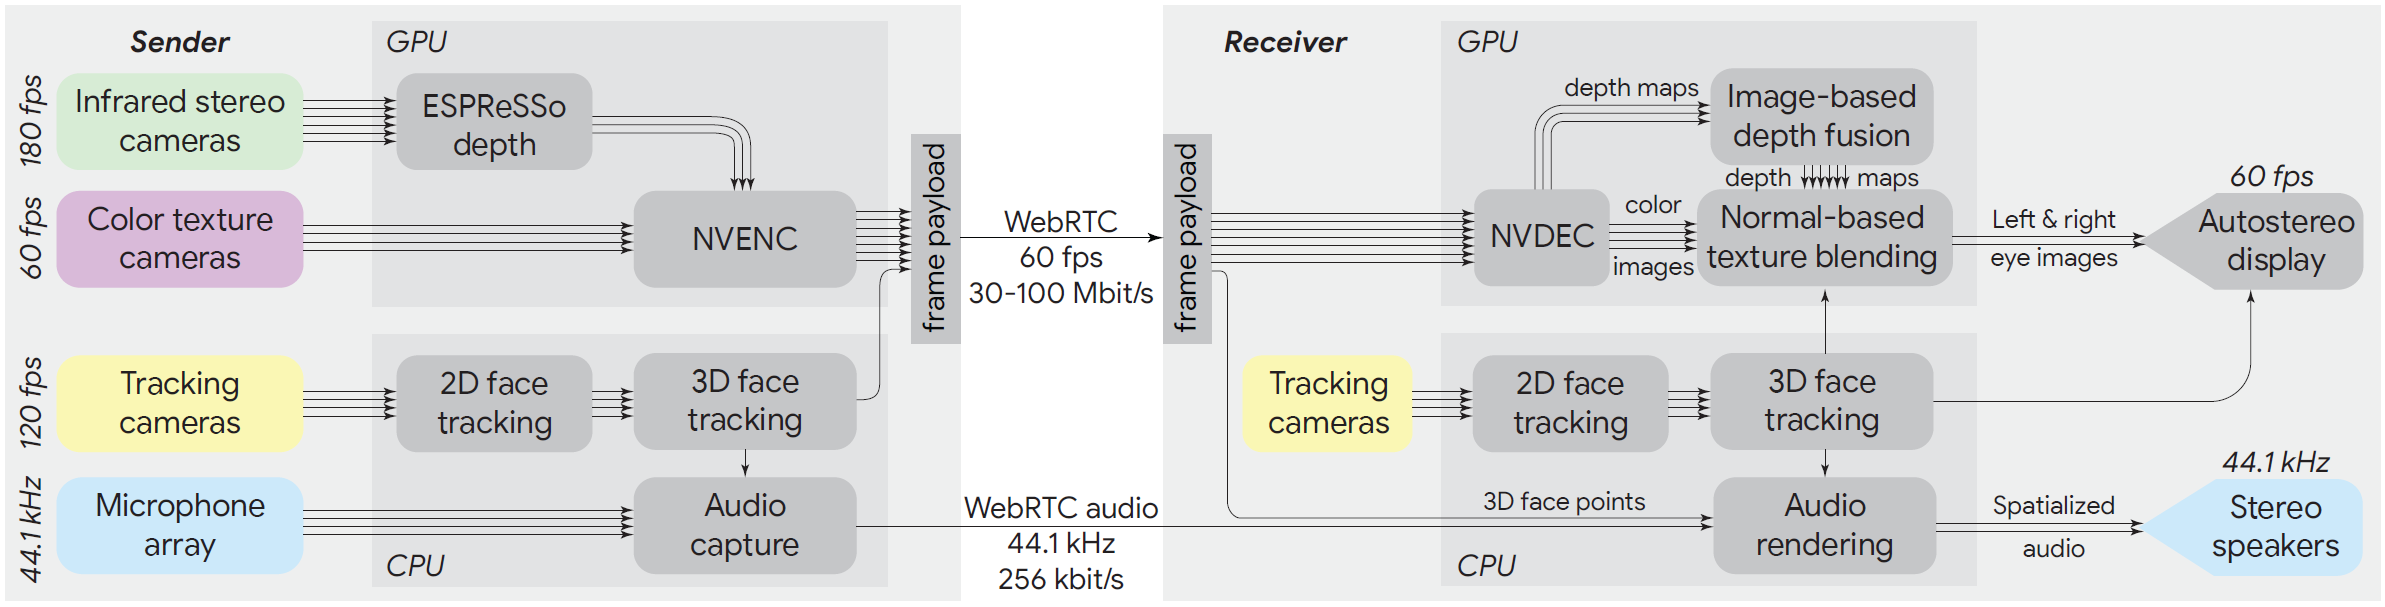
\includegraphics[width=1\columnwidth]{figures/project-starline-data-flow.png}
    \caption{Project Starline's Data Flow~\cite{lawrence_project_2021}}
    \label{fig:starline-data-flow}
\end{figure}

To capture a 3D video of the subjects, they use three groups of cameras they call ``pods," each with two infrared cameras and one color camera. The bottom pod contains an extra color camera zoomed into the face for higher resolution there. For stereo reconstruction, they use time-varying infrared pattern generators that create dot images only visible in infrared. They use windows of five infrared image pairs --- four with dot patterns and one with an infrared backlight --- to compute depth from space-time stereo using the ESPReSSo algorithm~\cite{nover_espresso_2018}. This algorithm takes as input infrared image pairs at 180 frames per second and computes synchronized output depth images at 60 frames per second. The infrared backlight is used to carve noisy background data from the stereo images and provides a reliable boundary for stereo estimation, improving accuracy at silhouette edges. In total, three depth and four color streams are sent over WebRTC using GPU video codec hardware. On the receiving side, after decompression, the system reprojects three depth images to the local subject's eye positions. A traditional volumetric fusion system~\cite{curless_volumetric_1996} would take these three depth images and fuse them into a voxel representation, extract the isosurface using marching cubes, and then render the triangles. Instead, Project Starline researchers use modern GPU hardware to eliminate the surface extraction step and raycast the voxels directly. This eliminates the additional data structures and unpredictable memory usage of a triangle mesh. However, it still requires a lot of GPU memory to store that voxel grid and a lot of memory bandwidth for the raycasting kernel to retrieve it. Hence they interleave the fusion and raycasting passes into a single kernel, fusing the depth images on the fly as they step through rays. This eliminates the need to store a voxel grid in GPU memory entirely, dramatically reducing memory usage and improving runtime by a factor of 6 over separate fusion and raycasting kernels. By eliminating this need to sample on an arbitrarily-aligned voxel grid, it can also reduce aliasing artifacts such as those sometimes seen along silhouette edges. Next, they project the color camera images onto the fused geometry and combine the colors using blend weights calculated from surface normals.

Their system doesn't work equally well for all scenes. Thin or frizzy hair is not well reconstructed as it falls below the minimum size of objects that their stereo system can detect. Similarly, fast motion can break up the reconstructed geometry, resulting in holes and incorrect texture projections. Eyeglasses also have thin geometric features and transparent surfaces that are missed by their 3D capture, causing incorrect texture projections. Despite these limitations, Project Starline conveys a strong sense of remote copresence.

Project Starline~\cite{lawrence_project_2021} is the first telepresence system that is demonstrably better than 2D videoconferencing, as measured using participant ratings (e.g., presence, attentiveness, reaction-gauging, engagement), meeting recall, and observed nonverbal behaviors (e.g., head nods, eyebrow movements). This milestone has been reached by maximizing audiovisual fidelity and the sense of copresence in all design elements, including physical layout, lighting, face tracking, multi-view capture, microphone array, multi-stream compression, loudspeaker output, and lenticular display. Their system achieves key 3D audiovisual cues (stereopsis, motion parallax, and spatialized audio) and enables the full range of communication cues (eye contact, hand gestures, and body language), yet does not require special glasses or body-worn microphones/headphones. Other contributions include a novel image-based geometry fusion algorithm, free-space dereverberation, and talker localization.






